\newcommand{\pname}{Levenberg-Marquardt}

\chapter*{Parameter Minimization using the \pname\ algorithm}
\setcounter{chapter}{1}
\emph{Do some fitting}
\section{Introduction}
The Levenberg-Marquardt plugin is used to fit an SBML model's parameters to experimental data.

The plugin has numerous properties to allow the user full control over the internal fitting engine, as well as
access to generated fitted data after a minimization session. In addition, various statistical properties, such as standardized residuals, Q-Q data, ChiSquare and reduced ChiSquare are made accessible to the user. The resulting parameter values also come with estimated confidence limits.

The current implementation is based on the lmfit C library by Joachim Wuttke\footnote{The package lmfit is distributed under the FreeBSD License:

--
  Copyright (c) 2013 Joachim Wuttke All rights reserved.
--}.


Plugin properties are documented in the next section.

\begin{landscape}
\section{Plugin Properties}
Available properties in the Levenberg-Marquardt plugin are listed in the table below.

%\begin{table}[ht]
\centering % used for centering table
\begin{longtable}{p{4cm} l p{3cm}  p{10cm}} % centered columns

Property Name & Data Type & Default Value  & Description \\ [0.5ex] % inserts table
%heading
\hline % inserts single horizontal line
SBML                            &   string              & N/A    &   SBML document as a string. Model to be used in the fitting. \\
ExperimentalData   				&	telluriumData 		& N/A    &   Input data.  \\
FittedData      				& 	telluriumData    	& N/A    &   Output data. \\
InputParameterList 				&	listOfProperties    & N/A    &   Parameters to fit. \\
OutputParameterList 			&   listOfProperties 	& N/A    &   List of fitted parameters. \\
Experimental\-DataSelectionList & 	stringList			& N/A    &   Species selection list for experimental data. \\
FittedDataSelectionList     	& 	stringList			& N/A    &   Selection list for model data. \\
Norm							&	double				& N/A    &   Norm of fitting. An estimate of goodness of fit. \\
Norms							&	telluriumData		& N/A    &   The norm is calculated throughout a fitting session. Each Norm value is stored in the 	\verb|Norms| (read-only) property. \\

ConfidenceLimits				&	listOfProperties	& N/A    &   Confidence limits for each fitted parameter. The confidence limits are calculated at a 95\% confidence level. \\

Hessian							&	matrix				& N/A    &   Hessian matrix. The Hessian is calculated using approximation at a found parameter minimum. \\
CovarianceMatrix				&	matrix				& N/A    &   Covariance matrix. Calculated as the inverse of the Hessian.\\
Residuals     					& 	telluriumData    	& N/A    &   Residuals data.  \\
StandardizedResiduals			&	telluriumData		& N/A    &   Standardized Residuals.\\
NormalProb\-abilityOfResiduals	&	telluriumData		& N/A    &   Normal Probability of Residuals.\\
ChiSquare						&	double				& N/A    &   The ChiSquare at the minimum.\\
ReducedChiSquare				&	double				& N/A    &   The Reduced ChiSquare at the minimum.\\
StatusMessage					&	string				& N/A    &   Message from the internal fitting engine, communicating the status of the obtained fit.\\
NrOfIter                        &   int                 & N/A    &   Number of iterations. \\[12pt]
\\[2pt]
\multicolumn{4}{p{19cm}}{The following properties are used internally by the fitting engine. They are pre-set with default values. Depending on the minimization problem at hand, they may need to be tweaked. } \\[12pt]
\hline %inserts single line
\\[2pt]
ftol                            &   double              & machine dep.          &   Relative error desired in the sum of squares. \\
xtol                            &   double              & machine dep.          &   Relative error between last two approximations. \\
gtol                            &   double              & machine dep.          &   Orthogonality desired between fvec and its derivs. \\
epsilon                         &   double              & machine dep.          &   Step used to calculate the Jacobian. \\
stepbound                       &   double              & 100.0                 &   Initial bound to steps in the outer loop. \\
patience                        &   double              & 100                   &   Used for setting maximum number of iterations, calculated as \verb|patience*(nr_of_parameters +1)|. \\

\hline %inserts single line
\caption{\pname\ plugin properties}
\label{table:lmfitPluginParameters}
\end{longtable}
%\end{table}

\end{landscape}


\section{The \texttt{execute(bool inThread)} function}
The \verb|execute()| function will start the \pname\ algorithm. Depending on the problem at hand, the algorithm may run for a long time.

The \verb|execute(bool inThread)| method supports a boolean argument indicating if the execution of the plugin work will be done in a thread, or not. Threading is fully implemented in the \pname\ plugin.

The inThread argument defaults to \textbf{false}.


\section{Plugin Events}
The Levenberg-Marquardt plugin are using all of a plugins available plugin events, i.e. the \emph{PluginStarted}, \emph{PluginProgress} and the \emph{PluginFinished} events.

The available data variables for each event are internally treated as \emph{pass through} variables, so any data, for any of the events, assigned prior to
the plugin's execute function (in the assignOn() family of functions), can be retrieved unmodified in the corresponding event function.

\begin{table}[ht]
\centering % used for centering table
\begin{tabular}{l l p{9cm}}

Event & Arguments & Purpose and argument types \\ [0.5ex] % inserts table
%heading
\hline % inserts single horizontal line
PluginStarted  	& 	void*, void*  & Signals to application that the plugin has started. Both parameters are \emph{pass through} parameters and are unused internally by the plugin.\\[0.5ex]
PluginProgress	& 	void*, void*  & Communicates progress of fitting. Both parameters are \emph{pass through} parameters and are unused internally by the plugin. \\[0.5ex]
PluginFinished	& 	void*, void*  & Signals to application that execution of the plugin has finished. Both parameters are \emph{pass through} parameters and are unused internally by the plugin.\\

\hline %inserts single line
\end{tabular}
\caption{Plugin events}
\label{table:lmfitPluginEvents}
\end{table}


\section{Python example}
The following Python script illustrates how the plugin can be used.

\begin{singlespace}
\lstinputlisting[label=plugin_lmfit_header,caption={Minimization example.},language=Python]{Examples/telLevenbergMarquardt.py}
\end{singlespace}

\begin{figure}[ht]
\centering
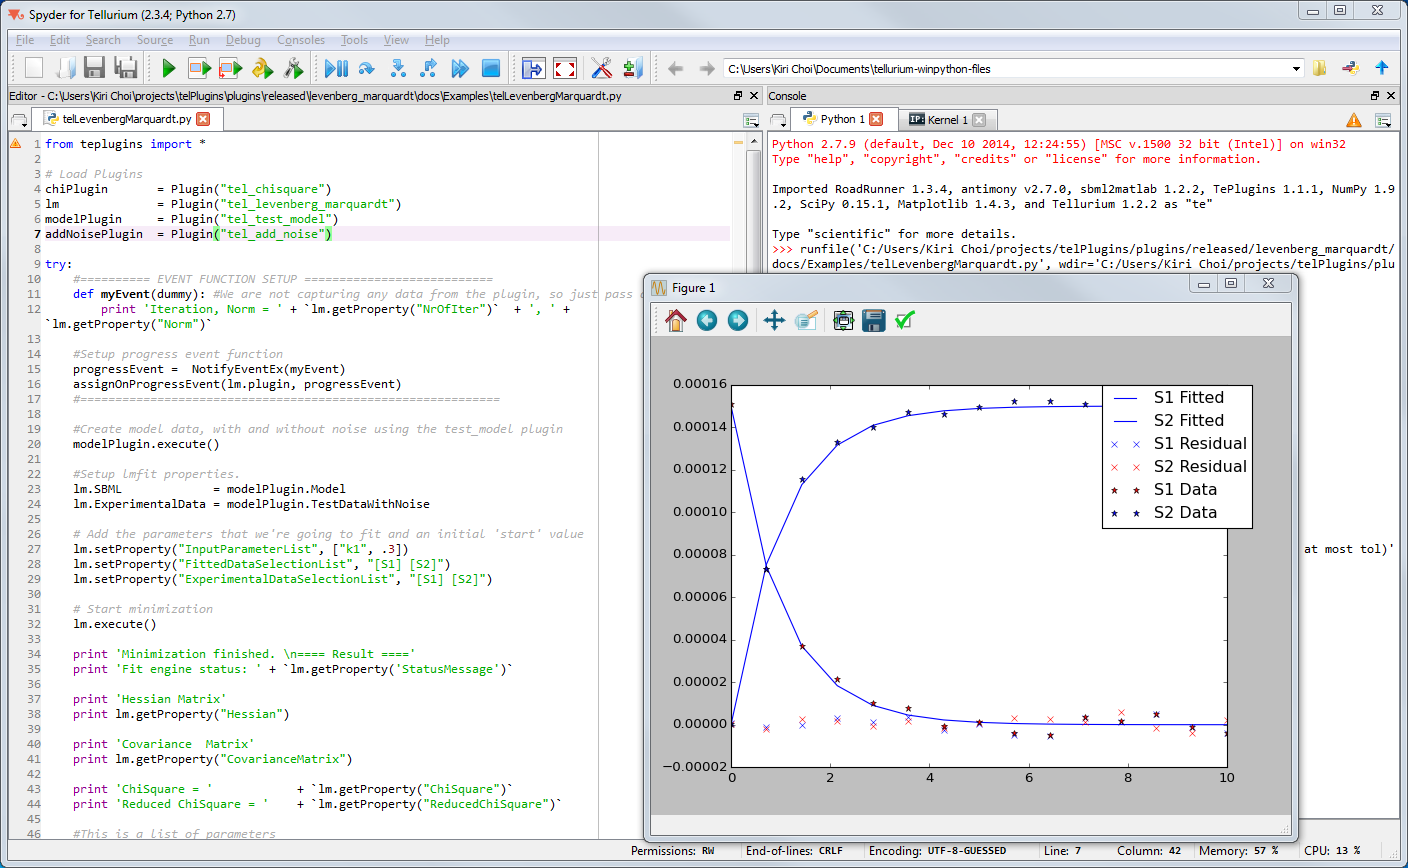
\includegraphics[width=\textwidth]{Minimization.png}
\caption{Typical output for the example script above.}
\label{fig:lmfitFig}
\end{figure}






